%%%%%%%%%%%%%%%%%%%%%%%%%%%%%%%%%%%%%%%%%%%%%%%%%%%%%%%%%%%%%%%%%%%%%%%%%%
%%%%%                          EPIGRAPHE                            %%%%%%
%%%%%%%%%%%%%%%%%%%%%%%%%%%%%%%%%%%%%%%%%%%%%%%%%%%%%%%%%%%%%%%%%%%%%%%%%%
\phantomsection 
\addcontentsline{toc}{section}{Épigraphe}
\addtocontents{toc}{\protect\addvspace{5pt}}

\lhead[\fancyplain{}{Épigraphe}]
      {\fancyplain{}{}}
\chead[\fancyplain{}{}]
      {\fancyplain{}{}}
\rhead[\fancyplain{}{}]
      {\fancyplain{}{Épigraphe}}
\lfoot[\fancyplain{}{}]
      {\fancyplain{}{}}
\cfoot[\fancyplain{}{\thepage}]
      {\fancyplain{}{\thepage}}
\rfoot[\fancyplain{}{}]%
     {\fancyplain{}{\scriptsize}}

%%%%%%%%%%%%%%%%%%%%%%%%%%%%%%%%%%%%%%%%%%%%%%%%%%%%%%%%%%%%%%%%%%%%%%%%%%
%%%%%                      Start part here                          %%%%%%
%%%%%%%%%%%%%%%%%%%%%%%%%%%%%%%%%%%%%%%%%%%%%%%%%%%%%%%%%%%%%%%%%%%%%%%%%%
\vspace*{-1cm} %5mm vertical space
% \lineskip=-\fboxrule
\begin{center}
	\shadowbox{
		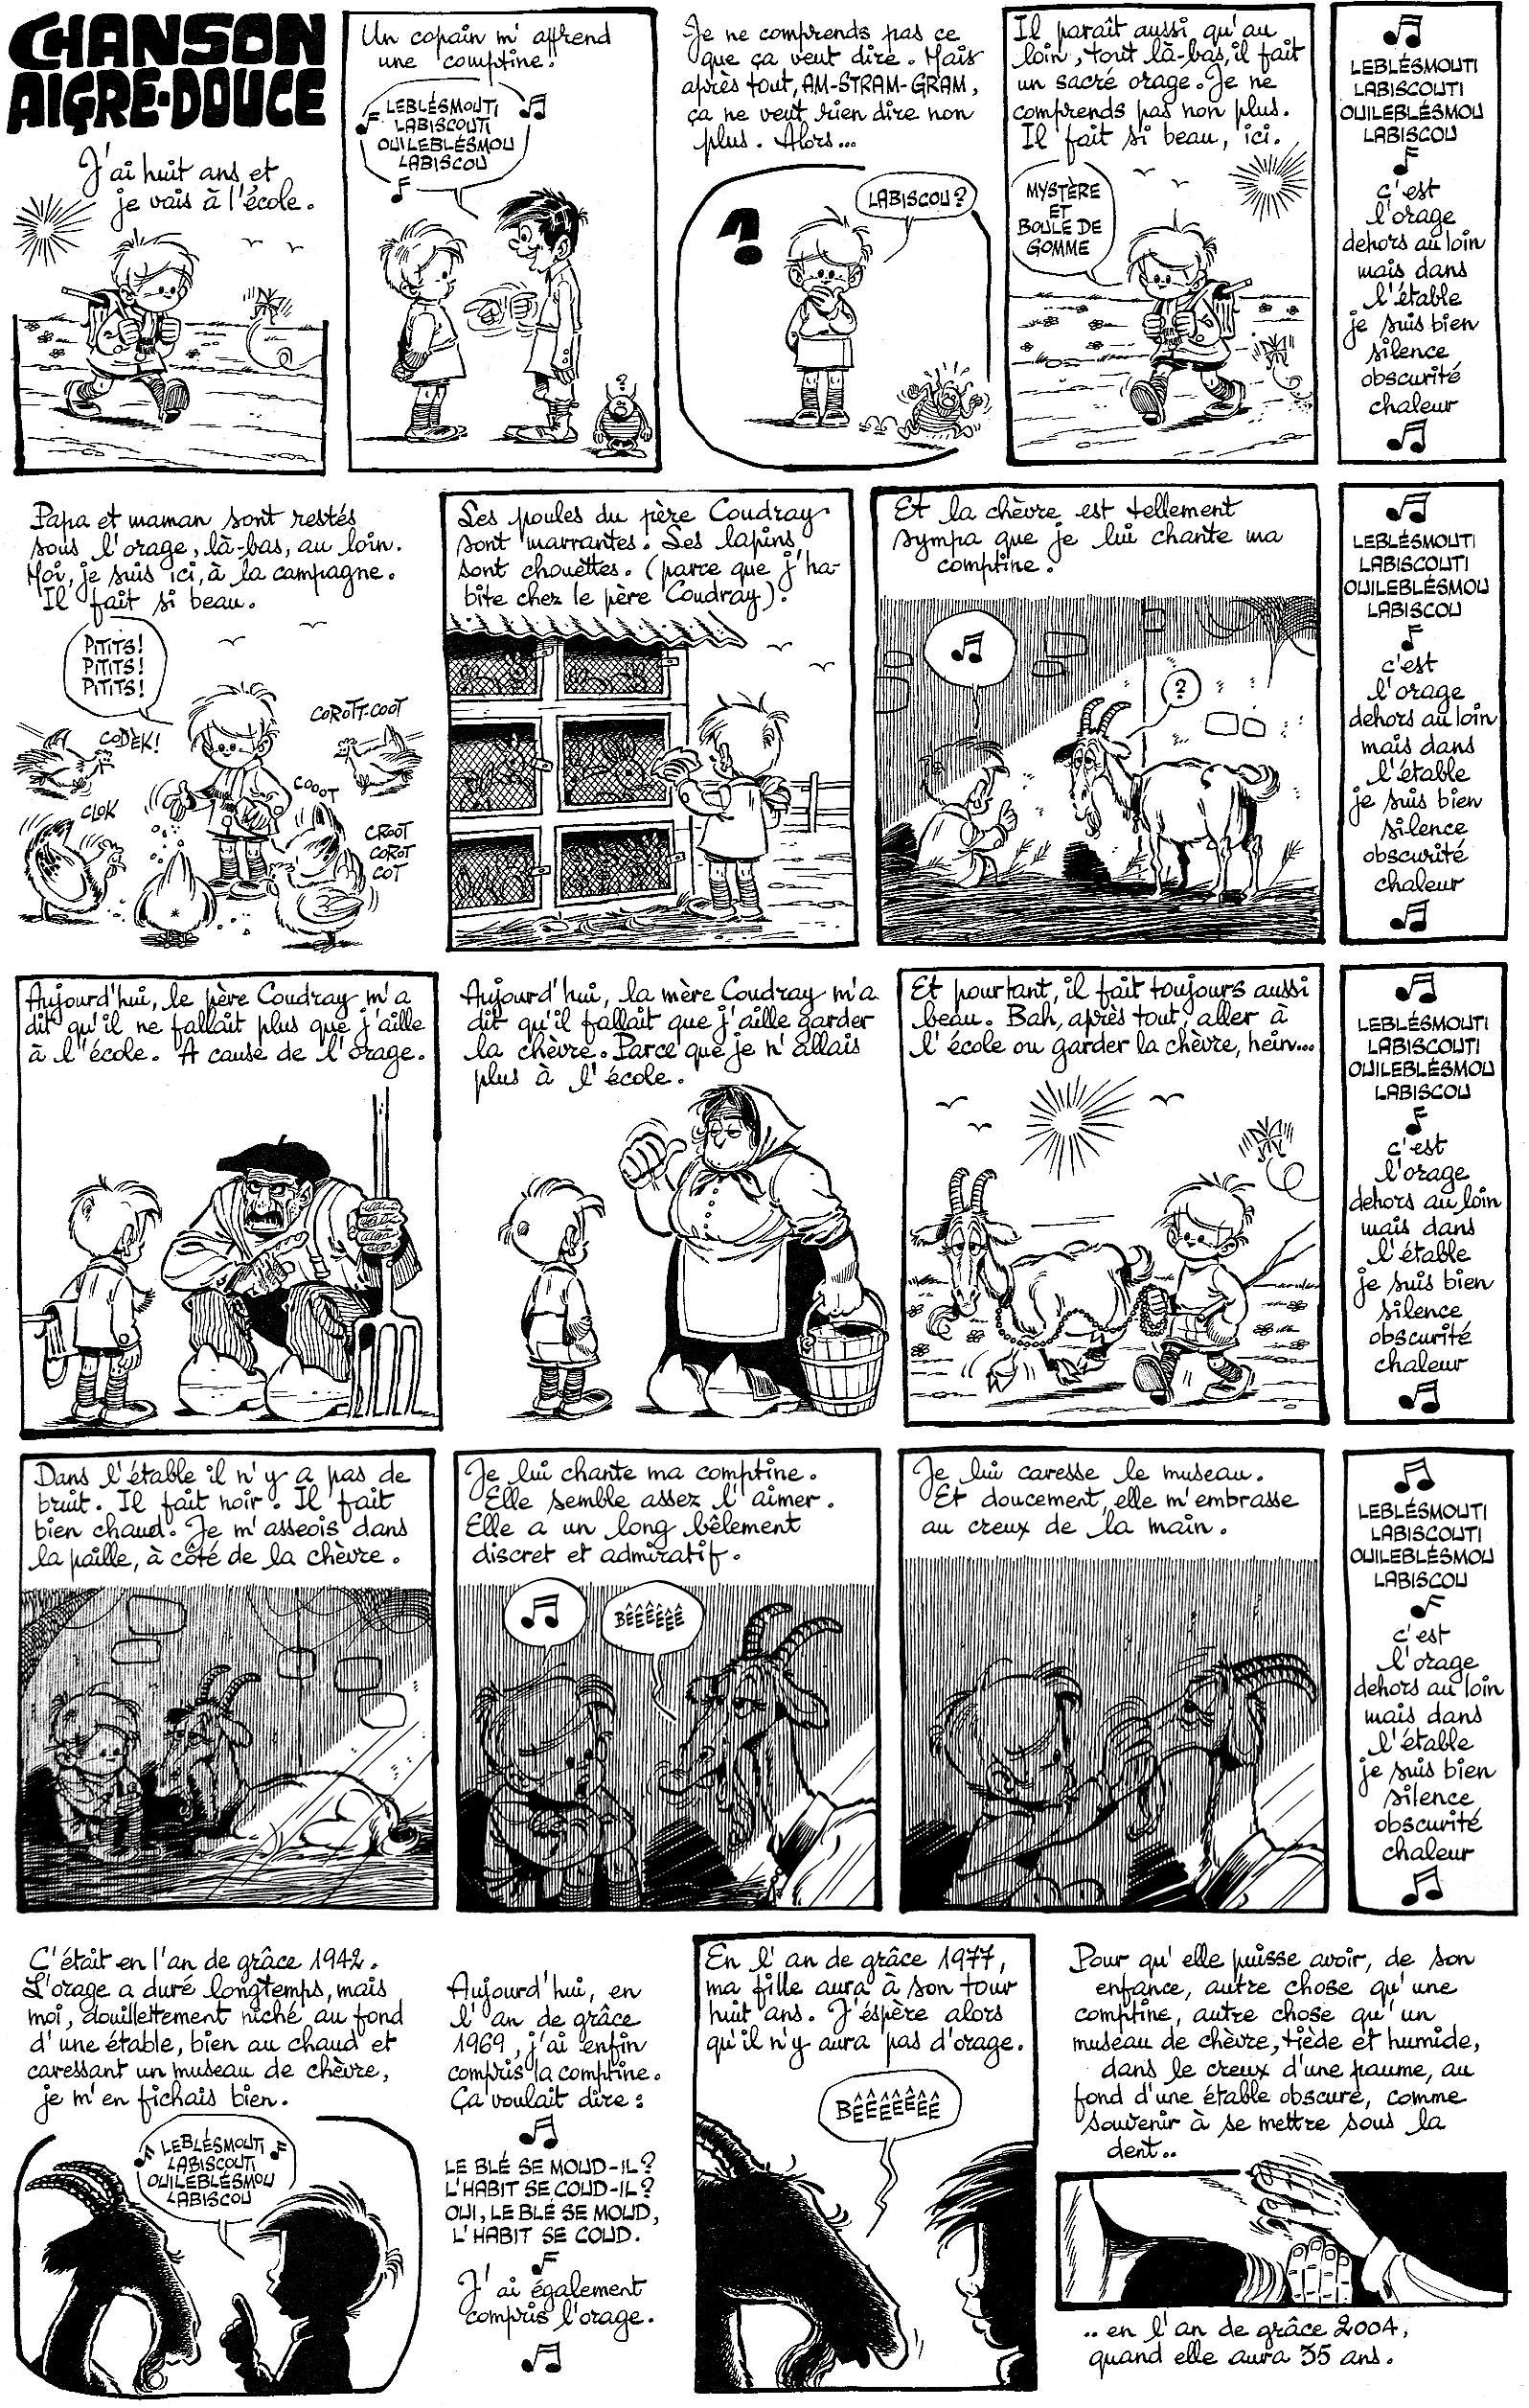
\includegraphics[width=0.96\textwidth,height=0.85\textheight]{../Intro/Figures/gotlib_chanson-aigre-douce.jpg} %keepaspectratio
	}
%\fbox{}
\end{center}
% \bigskip
% \bigskip
% \vfill
\vspace*{-3.5mm}
© Gotlib / Dargaud\footnote{Extraits de deux planches de Marcel Gotlib, publiées en Novembre 1969 dans le N°525 de l'hebdomadaire Pilote, puis dans la \textit{Rubrique-à-Brac Taume 2}, publiée aux éditions Dargaud.}  %\cite{gotlib_rubriqueabrac_1971}
% \vspace*{-1mm}

\vspace*{-3mm}
\begin{flushright}
\noindent
Mes grands-parents ont connu l'orage.\\
En 2000, j'avais huit ans, il n'y avait pas d'orage chez moi. Je suis allé à l'école.\\
En 2027, ma fille aura à son tour huit ans. J'espère qu'il n'y aura pas d'orage.\\
\end{flushright}
\vspace*{-1cm}
% ---
% Numéro 525 (27/11/1969) Complet
% RC 2p	Rubrique à brac	Chanson aigre–douce	Gotlib
% ---
% Marcel Gotlib « Sur l’air du Traderi-dera. Chanson aigre douce », Rubrique-A-Brac, Pilote, n° 525 du 27 novembre 1969. Extraits de planches reprises de l’album La Rubrique A Brac, publié aux éditions Dargaud, par La lettre de la Fondation de la Résistance, numéro 51, 2007, p. 28
% ---
% « Sur l’air du Traderi-dera. Chanson aigre douce », Rubrique-A-Brac, Pilote, n° 525 du 27 novembre 1969
% ---
% Fondation pour la Mémoire de la Shoah 5 décembre 2016 ·  La chanson aigre-douce (détail) Rubrique-à-brac, Pilote, 27 novembre 1969 © Gotlib - Dargaud
% ---
% Dans "La Chanson aigre-douce", Gotlib évoque la période de son enfance où il a dû vivre caché. (c) Dargaud
% ---
% Gotlib, Rubrique à Braque, Tome 2, ISBN : 2205005545 Éditeur : DARGAUD (07/06/1996)
% ---
% http://www.arac51.com/Dossier-du-Concours-National-de-la,364.html
% http://www.fondationresistance.org/documents/actualite_ped/Doc00012.pdf
% Marcel Gotlib « Sur l’air du Traderi-dera. Chanson aigre douce », Rubrique-A-Brac in Pilote n° 525 du 27 novembre 1969. Extraits de planches reprises de l’album La Rubrique A Brac, publié aux éditions Dargaud.
